\section{2020 年 11 月 22 日答疑记录}


\begin{example}
    如图所示, 已知边长为 $8$~米的正方形钢板有一个角被锈蚀, 其中 $AE=4$~米, $CD=6$~米. 为了合理利用这块钢板, 将在五边形 $ABCDE$ 内截取一个矩形 $BNPM$, 使点~$P$ 在边 $DE$~上.
    
    (1) 设 $MP=x$~米, $PN=y$~米, 将 $y$ 表示成 $x$ 的函数, 并求其定义域;
    
    (2) 求矩形 $BNPM$ 面积 $S$ 的取值范围.
    
    \begin{center}
        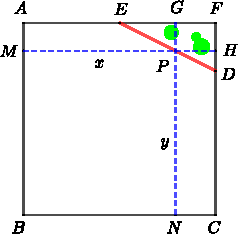
\includegraphics[scale=1]{2020-1206-1240-crop}
    \end{center}
    
\end{example}
\begin{solution}
    (1) 由题意, $\triangle DHP\backsim \triangle DEF$, 所以
    \[\frac{DH}{HP}= \frac{DF}{FE},\quad\text{即}\quad
        \frac{y-6}{8-x}= \frac{2}{4}.\]
    整理得, $y=\dfrac{20-x}2$, 且由图可知 $x\in[4,8]$.
    
    (2) 由 (1) 得, 
    \[S= xy= \frac12 x(20-x)\quad (\text{平方米}),\]
    且在 $[4,8]$ 上单调递增, 所以 $S\in[16,24]$ (平方米).
\end{solution}

\begin{example}
    (1) 若 $f(x)$ 为奇函数, 当 $x>0$ 时, $f(x)=x(1-\sqrt[3]{x})$, 求当 $x<0$ 时, $f(x)$ 的解析式;
    
    (2) 若 $f(x)$ 为偶函数, 当 $-1\leqslant x<0$ 时, $f(x)=\sqrt[5]{x}+1$, 求当 $0<x\leqslant 1$ 时, $f(x)$ 的解析式;
\end{example}
\begin{solution}
    以下过程较简略, 更详细的过程可参考 ``2020 年 11 月 14 日答疑记录'' 的例~\ref{exa:201206-1300} 方法一.
    
    (1) 因为 $f(x)$ 为奇函数, 所以当 $x<0$ 时,
    \[f(x)= -f(-x)= -(-x)(1-\sqrt[3]{-x})= x(1+\sqrt[3]{x}).\]
    
    (2) 因为 $f(x)$ 为偶函数, 所以当 $0<x\leqslant 1$ 时,
    \[f(x)= f(-x)= \sqrt[5]{-x}+1= -\sqrt[5]{x}+1.\]
\end{solution}

\begin{example}
    若函数 $f(x)$ 在 $\realnum$ 上为偶函数, 且当 $x>0$ 时, $f(x)=-x+1$, 求 $f(x)<-1$ 的解集.
\end{example}
\begin{solution}
    函数 $f(x)$ 在 $\realnum$ 上为偶函数, 表明其图形关于 $y$~轴对称. 直接根据对称性画图可知, $x\in(-\infty,-2)\cup(2,+\infty)$.
    
    \begin{center}
        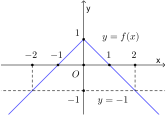
\includegraphics[scale=1]{2020-1206-1320-crop}
    \end{center}
\end{solution}

\begin{example}
    计算: (1) $\lg \sqrt[5]{100}$;\quad 
    (2) $\ln\sqrt[8]{\mathrm{e}}$;\quad
    (3) $9^{\log_3 4}$;\quad
    (4) $\log_9 27$;\quad (5) $\log_{\sqrt 6}36$.
\end{example}
\begin{solution}
    幂 (指数)、对数的运算法则见 ``2020 年 11 月 21 日答疑记录'' 的第二部分.
    
    (1) $\lg \sqrt[5]{100}= \lg 10^{\frac25}= \dfrac25$.\qquad
    (2) $\ln\sqrt[8]{\mathrm{e}}= \ln \mathrm{e}^{\frac18}= \dfrac18$.

    (3) $9^{\log_3 4}= \big(3^{\log_3 4}\bigr)^2= 4^2= 16$.\qquad
    (4) $\log_9 27= \dfrac{\ln 27}{\ln9}
        = \dfrac{3\ln3}{2\ln3}= \dfrac32$.
    
    (5) $\log_{\sqrt6}36= \dfrac{\ln 36}{\ln \sqrt6}
        = \dfrac{2\ln6}{\dfrac12\ln6}= 4$.
\end{solution}

\begin{example}
    ``$a+\dfrac1a>b+\dfrac1b$'' 是 ``$a>b$'' 的什么条件?
\end{example}
\begin{solution}
    利用 ``对勾'' 函数 $f(x)=x+\dfrac1x$ (参考 ``2020 年 10 月 31 日答疑记录'' 的第二个例题及其后的说明), 前一个条件等价于 $f(a)>f(b)$. 不妨只考虑 $a$, $b>0$ 的情况 (此时已可以得到结论). 由 $f(x)$ 的图形知, $f(a)>f(b)$ 与 $a>b$ 并不能互推 (即没有必然联系), 所以 ``$a+\dfrac1a>b+\dfrac1b$'' 是 ``$a>b$'' 的不充分且不必要条件.
    
    \begin{center}
        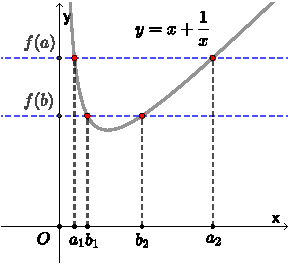
\includegraphics[scale=1]{2020-1206-1340-crop}
    \end{center}
\end{solution}

\begin{example}
    写出命题 ``$\exists\, x>0, x^3+x>0$'' 的否定.
\end{example}
\begin{solution}
    其否定为 ``$\forall\, x>0, x^3+x\leqslant 0$''.
\end{solution}

\begin{remark}
    (1) 形如 ``$\forall\, x\in M$, $p(x)$'' 的命题的否定为 ``$\exists\, x\in M$, $\neg p(x)$'', 而形如 ``$\exists\, x\in M$, $p(x)$'' 的命题的否定为 ``$\forall\, x\in M$, $\neg p(x)$''. 例如 ``$\forall\, x>1$, $x^2>1$'' 的否定为 ``$\exists\, x>1$, $x^2\leqslant 1$''.
    
    (2) 写命题的否定形式时, 一般只需要把原命题的判断词改为其否定形式, 比如 ``$=$'' 改为 ``$\neq$'', ``$>$'' 改为 ``$\leqslant$''. 例如, ``$x=1$'' 的否定为 ``$x\neq 1$'', ``$x<1$'' 的否定为 ``$x\geqslant 1$'' (并非 $x>1$), ``正整数 $x$ 至多为 $3$'' 的否定为 ``正整数 $x$ 至少为 4''.
\end{remark}

\begin{example}
    已知全集 $U=\{x\in\naturalnum\mid 0<x<6\}$, 集合 $A=\{x\mid x^2-6x+5=0\}$, $B=\{3,4\}$, 求 $(\complement_U A)\cap B$.
\end{example}
\begin{solution}
    由题意, $U=\{1,2,3,4,5\}$, $A=\{1,5\}$, 所以 $\complement_U A= \{2,3,4\}$, 而 $(\complement_U A)\cap B= \{3,4\}$.
\end{solution}